\documentclass[sigconf]{acmart}

\usepackage{booktabs} % For formal tables
\usepackage{listings}    
\usepackage{subcaption}
\usepackage{multirow}
% Copyright
%\setcopyright{none}
%\setcopyright{acmcopyright}
%\setcopyright{acmlicensed}
\setcopyright{rightsretained}
%\setcopyright{usgov}
%\setcopyright{usgovmixed}
%\setcopyright{cagov}
%\setcopyright{cagovmixed}
\usepackage{listings}
\usepackage{color}

\definecolor{dkgreen}{rgb}{0,0.6,0}
\definecolor{gray}{rgb}{0.5,0.5,0.5}
\definecolor{mauve}{rgb}{0.58,0,0.82}

\lstset{frame=tb,
	language=Java,
	aboveskip=3mm,
	belowskip=3mm,
	showstringspaces=false,
	columns=flexible,
	basicstyle={\small\ttfamily},
	numbers=none,
	numberstyle=\tiny\color{gray},
	keywordstyle=\color{blue},
	commentstyle=\color{dkgreen},
	stringstyle=\color{mauve},
	breaklines=true,
	breakatwhitespace=true,
	tabsize=3
}




\begin{document}
\title{Learning Cross Programming Language Mapping through Distributed Vector Representation}


\author{Nghi Bui}

\affiliation{%
  \department{School of Information Systems}
  \institution{Singapore Management University}
}
\email{dqnbui.2016@phdis.smu.edu.sg}

\author{Lingxiao Jiang}
\affiliation{%
  \department{School of Information Systems}
  \institution{Singapore Management University}
}
\email{lxjiang@smu.edu.sg}


% The default list of authors is too long for headers}
\renewcommand{\shortauthors}{Nghi et al.}


\begin{abstract}
Translation from a program written in a language to another is a common software engineering task. The programming languages differ from natural language in many aspects, thus the translation techniques for natural language are not usually applicable to a programming language. In order to tackle this problem, we propose a novel way to add more natural-like semantics feature into programming languages, thus making it feasible to apply the natural language techniques to the programming language translation problem. We adopt Word2Vec, a neural-based technique to learn vector representation of a word in the natural language, to learn the vector representation for tokens in a programming language. We consider the Word2Vec vector space for a pair of programming languages which can be translated from one to another, so called the shared embeddings. From the share embeddings, we can map the similar elements between languages accurately, thus the share embeddings space is served as a foundation for the program translation problem. Our empirical evaluation shows that our model can be used to map elements between languages accurately with high Mean Average Precision score. We also evaluate on a well-known real world task, the clone detection, we achieve a precision 84.2\% and recall 85.23\%.
\end{abstract}

%
% The code below should be generated by the tool at
% http://dl.acm.org/ccs.cfm
% Please copy and paste the code instead of the example below. 
%
\begin{CCSXML}
<ccs2012>
 <concept>
  <concept_id>10010520.10010553.10010562</concept_id>
  <concept_desc>Computer systems organization~Embedded systems</concept_desc>
  <concept_significance>500</concept_significance>
 </concept>
 <concept>
  <concept_id>10010520.10010575.10010755</concept_id>
  <concept_desc>Computer systems organization~Redundancy</concept_desc>
  <concept_significance>300</concept_significance>
 </concept>
 <concept>
  <concept_id>10010520.10010553.10010554</concept_id>
  <concept_desc>Computer systems organization~Robotics</concept_desc>
  <concept_significance>100</concept_significance>
 </concept>
 <concept>
  <concept_id>10003033.10003083.10003095</concept_id>
  <concept_desc>Networks~Network reliability</concept_desc>
  <concept_significance>100</concept_significance>
 </concept>
</ccs2012>  
\end{CCSXML}






\maketitle

\section{Introduction}

Distributional word representations can be learned from the distributional patterns in corpora. In the past, such representations can be constructed by counting co-occurrences, so that the features in one word's representation corresponded to other words. Word2vec (Mikolov et al., 2013c), which is a neural-based language model, is an alternative method for learning word representations. It uses language data to capture latent semantic features with respect to language modeling objective. The objective can be either to predict the context given a word or predict a word given a context. The representation learned by neural network models perform effectively in tackling various NLP tasks such as sentiment analysis, sentence parsing and neural machine translation (NMT).

Recently, NMT models have emerged as an alternative to statistical, phrase-based translation models, and achieved impressive translation performance. The objective of NMT is to generate an appropriate sentence in a target language T given a sentence in the source language S. The NMT system first aggregates the embedding of each word in the sentence through an encoder to build a "thought" vector, which is a sequence of number to represent the sentence meaning. and a decoder, then, processes the sentence vector to produce a translation. It raises a question: can we build a NMT model for programming languages? We have seen that at character-level, the neural network model is capable of writing Linux kernel after learning the entire Linux-based source code, as described in \cite{Karpathy}. 

Inspired by both of these, in this paper, we aim to build a shared token embeddings for programming languages. To the best of our knowledge, we are the first to use a neural-based language model to learn a share embedding cross-lingually. By learning a \textbf{billingual shared embedding space}, mapping similar elements between languages is achievable, thus this can be served as a foundation of NMT for programming languages. In our evaluations, we demonstrate the empirical strength of our model to represent a code fragment effectively for code clone detection task. We also show that by adding semantic keywords into the source code in the normalizing step, we can map the components of two languages accurately. 

\section{Background}

\subsection{A motivating example}
Each token in our model is represented by a 50 dimensional vector. To visualize our model, here we use t-Distributed Neighbor Embedding (t-SNE), a technique for dimensionality reduction that is particulary well suited for the visualization of high-dimensional datasets. 

In Figure 1, each pair of similar tokens are close together, e.g \textit{\textbf{if (\text{C\#})}} should be closest to \textit{\textbf{if (Java)}} and clusters with similar functionality should be located close to each other than other clusters, e.g the \textit{\textbf{if}} cluster should be closer to the \textit{\textbf{for}} cluster because both \textit{\textbf{if}} and \textit{\textbf{for}} are control statement.

\begin{figure}[t!]
	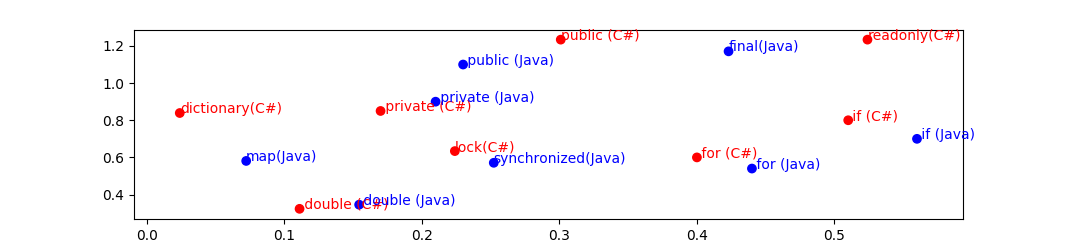
\includegraphics[width=0.55\textwidth]{example_bi2vec_tsne}
	\caption{A visualization of shared embeddings for between \text{C\#} and Java.}
	\label{fig:clf}
\end{figure}

\subsection{Background on Word2Vec}

Word2vec is a group of related models that are used to produce word embeddings. These models are shallow, two-layer neural networks that are trained to reconstruct linguistic contexts of words. Word2vec takes as its input a large corpus of text and produces a vector space, typically of several hundred dimensions, with each unique word in the corpus being assigned a corresponding vector in the space. Word vectors are positioned in the vector space such that words that share common contexts in the corpus are located in close proximity to one another in the space. Mikolov et al.\cite{mikolov2013distributed} introduce two variances of Word2Vec, which are Continuous Bag-of-Words (CBOW) and Skipgram. We show Skipgram model in Figure 2 as we use it in our work.

The training objective of the Skip-gram model is to find word representations that are useful for predicting the surrounding words in a sentence or a document. In other words, The Skipgram model aims to predict the word given the contexts. More formally, given a sequence of training words w1, w2, w3, . . . , wT , the objective of the Skipgram model is to maximize the average log probability

We show Skipgram model in Figure 2 as we use it in our work.

\begin{displaymath}
p(\textbf{a,t $|$ s}) = \prod_\text{j=1}^J p_{d}(\text{$a_{j}$ $|$ $a_{j\_}$,j}) p_{t}(\text{$t_{j}$ $|$ $s_{a_{j}}$})
\end{displaymath}

\begin{figure}[t!]
	
	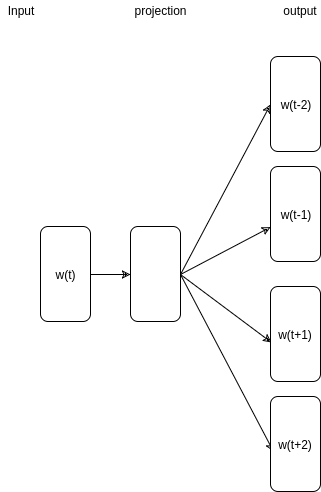
\includegraphics[width=0.20\textwidth]{skipgram}
	\caption{The Skip-gram model architecture. The training objective is to learn word vector representations that are good at predicting the nearby words.}
	\label{fig:clf}
\end{figure}

\section{Our Approach}
\subsection{Overview}
Figure 2 is the overview of our framework. There are 4 steps:
\begin{description}
	\item [$\bullet$] Clones alignment : Collect data crosslingually and align clones.
	\item [$\bullet$] Preprocessing: Preprocess the aligned data
	\item [$\bullet$] Token Alignment: Train the aligned clones to get the aligned information between tokens
	\item [$\bullet$] BiSkip Training: Get the shared embedding vector representation for all of the tokens in all languages.
\end{description}

\begin{figure}[t!]
	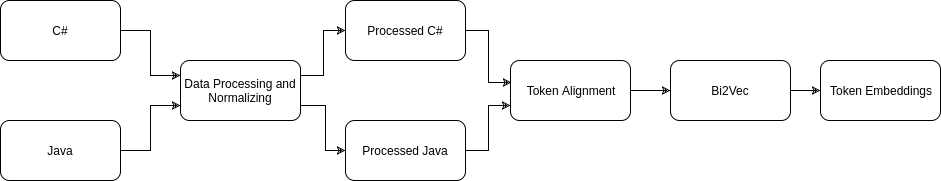
\includegraphics[width=0.45\textwidth]{steps}
	\caption{An overview of our framework}
	\label{fig:clf}
\end{figure}
 



\subsection{Data Normalizing}

In Natural Language Processing, the data normalizing step is a process to remove uninteresting contents from the data set and transform the rest into normalized comparison units. In our case, we are performing Programming Language Processing, besides removing uninteresting contents, we add more semantic features in order to 
This is the key step to learn the vector embedding cross-lingually since this step is to add more semantics to the training data. 

Figure 2 is an example of 2 similar implementations in cross languages, one is in \text{C\#}, and the other is in Java.

\begin{description}
	\item [$\bullet$] \textbf{Removing comments}: We remove all of the useless information such as comments out source code, special character, but not all of them. In order to keep as many semantic meanings as we can, we treat the operators as tokens that also need to learn the embeddings. Usually, the operators will be similar to the special character, to distinguish between them, we adopt Srcml \cite{collard2011lightweight} to parse the source code, so we can identify if a token is a language operator or just a special character.
	\item [$\bullet$] \textbf{Parsing}: We adopt Srcml[2], which is an XML representation of source code, where the markup tags identify elements of the abstract for the language.
	\item [$\bullet$] \textbf{Adding semantics}: Once we get the XML representation of the source code, we have the information of the element of the codes, we traverse the XML representation to add or replace code elements with predefined keywords to add more semantic meaning to the raw source code. The rules to add or replace code elements with keywords are presented in Table 1
	\item [$\bullet$] \textbf{Post processing}: camel case tokens and tokens with underscores are split by upper case letters and the underscore to reduce differences between programming styles.
\end{description}
Let's take the example of the first rule in Table 1 as a motivating example. We have code fragment \textbf{for(int i = 0; i $<$ 10; i++)}, which is a simple for loop with three elements, the initialization part, the condition part and the afterthought part. We apply rule 11 into the initialization, which transforms the variable i \textbf{i} into the fixed keyword \textbf{identifier}. Then we apply rule 11 and rule 12 to the condition part, by transforming \textbf{i} into \textbf{identifier} and \textbf{10} to \textbf{literal\_type number}. Finally, we apply rule 13, rule 15 to add the keyword \textbf{operator} before \textbf{++}. In Table 1, we selectively pick out some typical elements of programming languages to demonstrate our data normalizing process, the examples provided in the Table can be written in \text{C\#} or Java. 

Since the variable identifiers are the element with the highest number of appearance in the source code, and they are also project specific, means that an identifier can be anything so that it will add noises into the training phase, we replace all of the identifiers with a fixed keyword. In this paper, we use the keyword \textit{identifer}. For example, with the statement: \textit{int a}, we replace \textit{a} with \textit{identifier} to get \textit{int identifier}. There are also some project-specific elements like the name of methods, the name of classes, and types, but we decide to keep all of those elements as it. The first intuition behind this decision is that the appearance frequency of these elements is not as high as the variable identifiers, means that if a class name appears in some context, they tend to appear with approximately the same name in some other similar contexts. The second one is that the variable is usually used in a local scope, while the methods, the classes, and types are usually used in a global scope, means that they are defined once and are used everywhere in the project, so the developers tend to name them properly then the variables.


\begin{table*}
	\caption{Source code Transformation Rules.}
	\label{tab:freq}

	\begin{tabular}{p{2cm}|l|p{3cm}|p{4cm}|p{4cm}}
	
		\hline
		Element &Sub-Element&Rule&Example code&Applied Rules\\
		\hline
		Statements & if statement & add "condition" & if(x$>$5) y+=4 & if expr type int identifier operator $>$ literal\_type number expr\_stmt expr identifier operator += literal\_type number\\\cline{2-5}
		& for statement & add "condition","control" & for(int i=0;i$<$10;i++)  & for control init type int idenfier operator = number condition expr identifier operator $<$ literal\_type number identifier operator ++\\\cline{2-5}
	
		\hline
		Expressions & function call & add "call" & Console.WriteLine("out)  & expr\_stmt expr call Console Write Line argument literal\_type string\\\cline{2-5}
		\hline
		Declarations, Definitions and Initializations & variable declaration statement& add "decl\_stmt" & int i & decl\_stmt decl type int identifier\\\cline{2-5}
		& array declaration & add "array" & int[] numbers = new int[5]& decl\_stmt decl type int array identifier init operator new type int index literal\_type number \\\cline{2-5}
		& function declaration & add "function\_decl" & void doWork()& function\_decl void do Work \\\cline{2-5}
		& function definition & add "function" & void doWork() \{ \}& function void do Work \\\cline{2-5}
		& anonymous method & add "lambda" & delegate(System.Object o, System.EventArgs \{ \} & function void do Work \\\cline{2-5}
		\hline
		Others & inheritance list & add "super" & class Foo: Bar \{ \} & class Foo super Bar\\\cline{2-5}
		& inheritance list & add "super" & class Foo: Bar \{ \} & class Foo super Bar\\\cline{2-5}
		& constructor & add "constructor", "parameter\_list" & class Foo \{ Foo(int i)\{\}\} & class Foo constructor Foo parameter\_list parameter decl type int identifier\\\cline{2-5}
		& destructor & add "destructor", "parameter\_list" & class Foo \{  Foo()\{\}\} & class Foo destructor Foo\\\cline{2-5}
		\hline
	\end{tabular}
\end{table*}
\subsection{ Unsupervised token alignment}

Once we finish normalizing our training data, we want to learn a shared embedding space between tokens crosslingually rather than just monolingually.

In order to do that, we need to obtain aligned information from such languages. We briefly review the sequence-based token alignment models. Generally, the token alignment model are generative models of the form p(\textbf{t $|$ s}) = $\displaystyle\sum_{a} p(\textbf{a,t $|$ s})$, where $\textbf{s} = (s_{1},..., s_{J})$ is the source sentence, $\textbf{t} = (t_{1},..., s_{J})$ is the target sentence and $\textbf{a} = (a_{1},..., a_{J})$ is the asymmetric alignment which specifies the position of a token in source language aligned to each target language. The model factors in the following way:
\begin{displaymath}
p(\textbf{a,t $|$ s}) = \prod_\text{j=1}^J p_{d}(\text{$a_{j}$ $|$ $a_{j\_}$,j}) p_{t}(\text{$t_{j}$ $|$ $s_{a_{j}}$})
\end{displaymath}

where \text{j\_} is the position of the last non-null-aligned target token before position j. Bekerley aligner (Liang et al. \cite{liang2006alignment}) is a joint training approach, while the source language and target language play a symmetric role in the word alignment task, sequence-based models are asymmetric,they are generative models of the form p(\textbf{t $|$ s})(S $\rightarrow$ T) or p(\textbf{s $|$ t})(T $\rightarrow$ S) by reversing the roles of source and target. This suggests that two models make different types of errors that can be eleminated upon intersection. Figure 2 shows an example alignment of tokens of code fragments between \text{C\#} and Java code.

\begin{figure}[t!]
	
	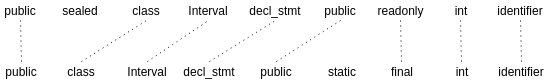
\includegraphics[width=0.45\textwidth]{alignment}
	\caption{Sample alignment of code fragments between \text{C\#} and Java code, both the fragments have already been processed.}
	\label{fig:clf}
\end{figure}

\subsection{The Billingual Skipgram Model}
The motivation behind the billingual skip gram (BiSkip) model is to learn a shared embedding space between tokens crosslingually rather than just monolingually in the standard skipgram model. Rather than just predicting the tokens in the source language, they use the tokens in the source language to additionally predict their aligned tokens in the target languages. Imagine that if we know that the token \textit{readonly} in \text{C\#} is aligned to and has the same meaning as the token \textit{final} in Java in Figure 3, we can simply substitute \textit{readonly} and use \textit{final} to predict the surrounding tokens such as \textit{int} and \textit{public}. 

Given an alignment link between a token $t_{1}$ in a language $l_{1}$ and a token $t_{2}$ in another language $l_{2}$, the BiSkip model uses the token $t_{1}$ to predict the surrounding tokens of the token $t_{2}$ and vice versa. We can think of this BiSkip model as training four skipgram models jointly which predict tokens betwwen the follow pairs of languages: $l_{1} \rightarrow l_{1}, l_{2} \rightarrow l_{2}, l_{1} \rightarrow l_{2}, l_{2} \rightarrow l_{1}$.

In order to train the BiSkip model, we need the token alignment information. There are two variants of the BiSkip model: (a) BiSkip-UnsupAlign where we don't have the alignment information, thus the alignment information need to be learned unsupervisedly and (b) BiSkip-MonoAlign where we already have the monotonic alignments between words across languages. In our case, we do not have the word alignment information, so we use the BiSkip-UnsupAlign where we can utilize unsupervised align information learned by the Bekerley aligner (Liang et al., 2006), which are presented briefly in Section 3.2.


\begin{figure}[t!]
	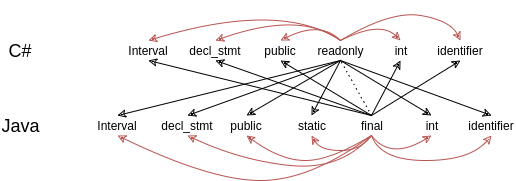
\includegraphics[width=0.35\textwidth]{biskip_align}
	\caption{Billingual Skipgram Model - besides predicting within languages, the model also predict crosslingually based on the alignment information \text{C\#} and Java}
	\label{fig:clf}
\end{figure}

\section{Experiments}
\subsection{Data}
We collect data from 12 open source projects crosslingually. With the intuition that the different implementations of the same project in different languages will contain the same logic, thus files with the same name will contain the same logic, so they are aligned to each other. In natural language processing, such information is called aligned sentences or aligned documents. Here we use another terminology, but with the same concept, we call them "clones". For example, take the \text{C\#} implementation and Java implementation of Lucence, there are 400 cs files in the C\# implementation, and there are 300 java files, there are only 100 pairs of files between implementations that are cloned of each other. We get 4000 pairs of clones over 12 projects and we normalize all the pairs.
\subsection{Training}
We use the following settings: stochastic gradient descent with a default learning rate 0.025, negative sampling with 30 samples, skipgram with context window of size 10, and a subsampling rate of value 1e-4. All models are trained for 10 epochs and the learning rate is decayed to 0 once training is done. In Natural Language, the number of words is usually large and we need a large dimension (range from 100 to 300) to capture the semantic meaning of the word, while the number of tokens in Programming Language is relatively small, so we choose 50 as the dimension size.
\subsection{Evaluation Tasks}
We evaluate our architectures on 3 aspects: token similarity, phrase similarity.
\subsubsection{Component Similarity}
This task measures the semantic qualitfy of the learned token vectors crosslingually. In software engineering, a program can be constructed from: expression, declaration and statements. We want to evaluate how we can match such elements between different languages together.
\subsubsection{Clone detection}
To evaluate the impact of our model on real world tasks, we evaluate the diff dataset from (Cheng at al., 2016). The dataset contains of 1000 pairs of diff, one from C\# and the other is from Java, which have been labeled either cloned or non-cloned. 

\subsection{Result}
\subsubsection{Nearest Neighbor Tokens}
This task measures the semantic quality of the learned token vectors crosslingually. Our list of words include {if, exception, float}.
\begin{table*}
	\caption{Nearest neighbor tokens}
	\label{tab:freq}
	
	\begin{tabular}{cccccc}
		
		\hline
		\multicolumn{2}{c}{if(Java)}  & \multicolumn{2}{c}{exception(Java)} & \multicolumn{2}{c}{float(C\#)} \\
		\hline
		 C\# & Java & C\# & Java & C\# & Java \\
		\hline
		 if & if & throw & exception & float & float \\
		 break & \&\& & exception & throw & weight & double \\
		 while &  $||$ & try & throwable & weight & similarity \\
		 == & continue & catch & catch & double & weight \\
		 else & while & finally & catch & comparator & score\\
	
		\hline
	\end{tabular}
\end{table*}
\subsubsection{Elements matching}
In software engineering, a program can be constructed from: expression, declaration and statements. In this task, we want to evaluate how we can match such elements between different languages together. We selectively pick elements from real source code in open source projects, then we compare the similarity of such elements.


\begin{table*}
	\caption{Elements Matching Result}
	\label{tab:freq}
	
	\begin{tabular}{p{2cm}|l|p{5cm}|p{5cm}|p{1cm}}
		
		\hline
		Element &Sub-Element& Java code &C\# code& Cosine Similarity\\
		\hline
		Expression & bit expression & c = a $<<$ 2; & c = a $<<$ 2; & 0.900 \\\cline{2-5}
		& literal expression & string s = "cat"; & string s = "cat";  & 0.918\\\cline{2-5}
		& logical expression & a\&\&b; & a\&\&b;  & 0.812\\\cline{2-5}
		& numeric expression & 45 + 20.2 + 10; & 45 + 20.2 + 10;  & 0.869\\\cline{2-5}
		& assignment expression & int a = b; & int a = b;  & 0.9438\\\cline{2-5}
		& object creation expression & Object o = new Object (); & Object o = new Object ();  & 0.937\\\cline{2-5}
		& string expression & "abc" + "cde"; & "abc" + "cde";  & 0.8\\\cline{2-5}
		& conditional expression & a == b; & a == b;  & 0.917\\\cline{2-5}
		\hline
		
	
		Declaration & field declaration & public static int i = 10; & public static int i = 10; & 0.934 \\\cline{2-5}
		& interface declaration & public interface CardCredit {} & public interface CardCredit {} & 0.79\\\cline{2-5}
		& array declaration & int[] numbers = new int[5]; & int[] numbers = new int[5];  & 0.91\\\cline{2-5}
		& method declaration & void doWork(); & void doWork();  & 0.839\\\cline{2-5}
		& type declaration & public class Inference & public class Inference  & 0.833\\\cline{2-5}
		& variable declaration & int i; & int i;  & 0.845\\\cline{2-5}
		& class and constructor declaration & class Foo \{ Foo() \{\}\} & class Foo \{ Foo() \{\}\}  & 0.956\\\cline{2-5}
		
		\hline
		Statement & if statement & if ( i $>$ 0 ) \{ y = x $/$ i;\} & if ( i $>$ 0 ) \{ y = x $/$ i;\} & 0.902 \\\cline{2-5}
		& for statement & for(int i = 0; i < 10;i++)\{\} & for(int i = 0; i < 10;i++)\{\} & 0.908\\\cline{2-5}
		& do statement & do \{ number ++;\} while (number $<=$ 20); & do \{ number ++;\} while (number $<=$ 20);  & 0.865\\\cline{2-5}
		& while statement & while (number $<=$ 20) \{ number++; \} & while (number $<=$ 20) \{ number++; \}  & 0.934\\\cline{2-5}
		& variable declaration statement & int myInt; & int myInt; & 0.962\\\cline{2-5}
		& return statement & return i; & return i;  & 0.912\\\cline{2-5}
		& try statement & try \{\} catch (Exception e)\{\} & try \{\} catch (Exception e)\{\}  & 0.843\\\cline{2-5}
		& switch statement & switch (c) \{ case 'A': capa++; case 'a': lettera++; default :total++;\} & witch (c) \{ case 'A': capa++; case 'a': lettera++; default :total++;\}  & 0.912\\\cline{2-5}
	\end{tabular}
\end{table*}

\subsubsection{Clone Detection}
For each diff, we perform normalizing step (Section 3.1) to get the normalized version of the code, here we call it as token stream. Then we get the vector representation of the token stream by averaging token vectors for all tokens, once we get the vector representation, we calculate the similarity between vectors by using the cosine similarity metric. We plot the probability (Figure 5) density function of a distribution of cosine similarity for all pairs of diff. Here we want to find the decision boundary to seperate 2 groups, then our problem become the classification problem, the cosine similarity is the only feature for the model. We use the Logistic Regression as a simple classifier for this problem.

\begin{figure}[t!]
	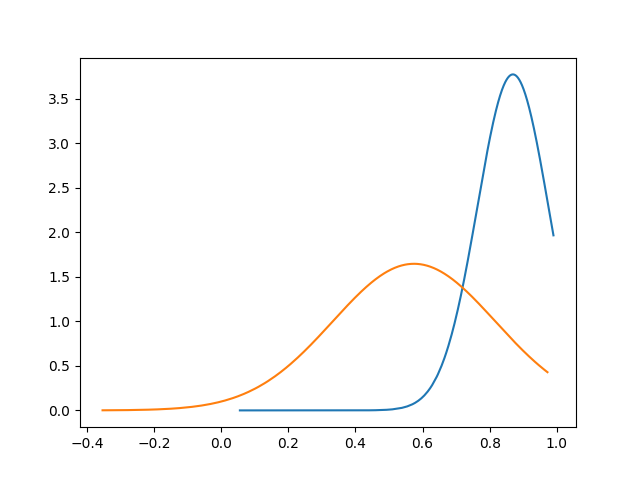
\includegraphics[width=0.45\textwidth]{clone_distribution}
	\caption{Plot of Probability Density Function of a distributon of cosine similarity for all pairs of diffs - The blue curve indicates the  probability density function of cosine similarity of the cloned pairs. The yellow curve is for the non-clone pairs.  }
	\label{fig:clf}
\end{figure}


\begin{table*}
	\caption{Clone detection result}
	\label{tab:freq}
	
	\begin{tabular}{c|ccccccc}
		
		\hline
		Projects&Antlr&Cordova &DataSax&Factual&Log4j&	Lucene&	Zeromq\\
		\hline
		Precision&	82.30\% &	83.60\%&	83.20\%&	85.23\%&	84.56\%&	85.12\%&	81.15\%\\
		Recall&	82.30\%&	84.22\%&	83.20\%&	85.23\%&	83.92\%&	85.12\%&	81.15\%\\
		\hline
	\end{tabular}
\end{table*}

\subsection{Discussion}
As described in (Mikolov at at.; 2013c), the Skipgram model (SG) works well with small amount of the training data, represents well even rare words or phrases, while the Continuos Bag of Words model (CBOW) is several times faster to train than the skip-gram and slightly better accuracy for the frequent words. Since CBOW considers one target word and many context words, the task here is to predicting the word given its context, it needs a bigger dataset to train for target vectors compared to datasets used in SG. In other words, a dataset with short sentences but with high number of samples is suitable for the CBOW model. On the other hand, the Skipgram model (SG) is designed to predict the context, so it needs a dataset with long sentences and low number of samples due to many target words for single context word. In our case, a file (.java or .cs) are usually quite long, compare to a normal sentence in Natural language, then the SG is a more suitable model in this case. 

Recently, Google Brain releases Neural Machine Translation tutorial \cite{Thang} for TensorFlow that gives the reader the ability to build a competitive translation model from scratch. As machine translation of human language is largely improved and successful by employing deep neural network, it is a reasonable target to do the same thing for programming language because we've seen that character-level is capable of writing Kinux kernel after learning the entire Linux base source code, as described in \cite{}. We believe that this can be a good foundation for a neural network-based programming language translation, which is a more sophisticated task. 

\section{Conclusions}
This work proposes an approach to learn the elements mapping between languages. By utilizing the clones of cross language implementation for the same logic, we can learn the alignments unsupervisedly, then we can learn the share embeddings between languages. With not a very large dataset, we show that we can still map the elements between languages accurately. This can be served as a foundation for more complicated tasks, such as programming language translation. In the future, we want to collect more data in order to train a more accurate embeddings, then we want to adopt the embeddings as a part of a neural network-based program translation.



\begin{acks}

\end{acks}


\bibliographystyle{ACM-Reference-Format}
\bibliography{sample-bibliography} 

\end{document}
